\documentclass[conference]{IEEEtran}
\IEEEoverridecommandlockouts
\usepackage{cite}
\usepackage{amsmath,amssymb,amsfonts}
\usepackage{algorithmic}
\usepackage{graphicx}
\usepackage{textcomp}
\usepackage{xcolor}
\usepackage{booktabs}
\usepackage{array}
\usepackage{tikz}
\usetikzlibrary{shapes.geometric, arrows.meta, positioning, fit, backgrounds}
\usepackage{listings}
\usepackage[portuguese]{babel}
\usepackage[utf8]{inputenc}
\usepackage[hidelinks]{hyperref}
\graphicspath{{./figs/}}
\def\BibTeX{{\rm B\kern-.05em{\sc i\kern-.025em b}\kern-.08em
    T\kern-.1667em\lower.7ex\hbox{E}\kern-.125emX}}

% -------- Estilo dos blocos de código (TypeScript/Deno) --------
\definecolor{codebg}{HTML}{F7F7F9}
\definecolor{codekw}{HTML}{0033B3}
\definecolor{codestr}{HTML}{067D17}
\definecolor{codecom}{HTML}{8C8C8C}
\definecolor{codetype}{HTML}{B58900}
\lstdefinelanguage{TypeScript}{
  keywords={const,let,var,function,return,if,else,for,while,import,from,export,default,async,await,new,typeof,interface,type,number,boolean,string,void,null,undefined,as,Number},
  keywordstyle=\color{codekw}\bfseries,
  ndkeywords={Response,Request,Uint8Array,Array,Promise},
  ndkeywordstyle=\color{codetype}\bfseries,
  sensitive=true,
  comment=[l]{//},
  morecomment=[s]{/*}{*/},
  commentstyle=\color{codecom}\itshape,
  stringstyle=\color{codestr},
  morestring=[b]",
  morestring=[b]'
}
\lstset{
  language=TypeScript,
  backgroundcolor=\color{codebg},
  basicstyle=\ttfamily\footnotesize,
  breaklines=true,
  showstringspaces=false,
  numbers=left,
  numberstyle=\tiny\color{codecom},
  numbersep=6pt,
  frame=single,
  rulecolor=\color{black!25},
  framesep=4pt,
  xleftmargin=12pt,
  aboveskip=8pt,
  belowskip=4pt,
  columns=fullflexible,
  keepspaces=true
}

\begin{document}

\title{Edge Functions do Supabase:\\ Geração \textit{Serverless} de Números Primos}

\author{\IEEEauthorblockN{1\textsuperscript{st} Enrico Nunes}
\IEEEauthorblockA{\textit{Mestrado em Engenharia Informática}\\
\textit{Universidade da Beira Interior}\\
Covilhã, Portugal\\
enrico.nunes@ubi.pt}
\and
\IEEEauthorblockN{2\textsuperscript{nd} Marcos Assunção}
\IEEEauthorblockA{\textit{Mestrado em Engenharia Informática}\\
\textit{Universidade da Beira Interior}\\
Covilhã, Portugal\\
marcos.assuncao@ubi.pt}
}

\maketitle

\IEEEpubidadjcol
\renewcommand{\thefootnote}{}
\footnotetext{Código-fonte e \textit{scripts} de teste disponíveis em \url{https://github.com/enriconunes/serverless-function-ubi}.}
\renewcommand{\thefootnote}{\arabic{footnote}}

\begin{abstract}
A computação \textit{serverless} eliminou a fronteira entre escrever uma função e disponibilizá-la na Internet, transferindo para o fornecedor de nuvem a responsabilidade de provisionar, escalar e manter a infraestrutura. Este trabalho concretiza essa abordagem implementando uma função que devolve todos os números primos inferiores a $n$, exposta como \textit{endpoint} HTTP através das \textit{Edge Functions} do Supabase. A função é escrita em TypeScript sobre o \textit{runtime} Deno e implantada na \textit{edge network} do fornecedor. O relatório descreve o conceito de \textit{Function as a Service}, compara as principais plataformas do mercado, justifica a escolha do Supabase e detalha o processo de desenvolvimento e \textit{deployment}, incluindo o algoritmo utilizado.
\end{abstract}

\begin{IEEEkeywords}
\textit{Serverless}, \textit{Function as a Service}, Supabase, \textit{Edge Functions}, Deno, \textit{cold start}, números primos.
\end{IEEEkeywords}

%=================================================================
\section{Introdução}
%=================================================================
Durante a última década, a forma como o software é executado em nuvem deslocou-se progressivamente do servidor para a função. Onde antes era necessário aprovisionar uma máquina virtual e mantê-la em execução à espera de pedidos, hoje basta enviar uma função para uma plataforma que se encarrega de a invocar quando, e apenas quando, alguém a chama. Este modelo, designado \textit{serverless}, não significa a ausência de servidores; significa apenas que estes deixam de fazer parte do modelo mental do programador \cite{baldini2017,castro2019}.

Neste trabalho concretiza-se um caso de uso simples mas suficientemente ilustrativo: uma função que recebe um número natural $n$ e devolve todos os primos inferiores ou iguais a $n$. A escolha do problema é deliberada. O cálculo é puramente determinístico e dependente de CPU, sem acessos a base de dados nem dependências externas, o que permite que a medição posterior de latência e \textit{cold start} reflita o comportamento da plataforma e não o de serviços auxiliares.

A função foi implementada em TypeScript, executada sobre o \textit{runtime} Deno, e implantada nas \textit{Edge Functions} do Supabase. O relatório está organizado nas secções habituais: conceitos de \textit{serverless} e \textit{Function as a Service} (II), panorama das plataformas disponíveis (III), justificação da escolha do Supabase e descrição da implementação e \textit{deployment} (IV), seguida da análise de desempenho (V), conclusões (VI) e referências.

%=================================================================
\section{Computação \textit{Serverless} e \textit{Function as a Service}}
%=================================================================
A computação \textit{serverless} é um modelo de execução em que o fornecedor de nuvem atribui dinamicamente os recursos necessários a cada invocação e cobra apenas pelo tempo efetivamente consumido, em geral medido à escala dos milissegundos. O programador deixa de gerir máquinas, sistemas operativos ou \textit{runtimes} e passa a entregar unidades muito mais pequenas de código \cite{baldini2017,jonas2019}.

Dentro deste paradigma, \textit{Function as a Service} (FaaS) é a forma de exposição mais difundida. Uma função FaaS é uma peça de código sem estado, com um ponto de entrada bem definido, acionada por um evento: um pedido HTTP, uma mensagem numa fila, a escrita num \textit{bucket} de armazenamento ou um agendamento temporal. O modelo é resumido por três propriedades operacionais.

\textbf{Escalabilidade automática.} O fornecedor instancia tantas cópias da função quantas as necessárias para absorver a carga, e remove-as quando esta cai para zero. Esta elasticidade quase instantânea é o principal argumento técnico do modelo.

\textbf{Pagamento por uso.} A cobrança incide sobre o número de invocações e sobre o produto entre tempo de execução e memória alocada. Picos de utilização e funções pouco invocadas têm um custo proporcional, sem o desperdício de máquinas semipreenchidas.

\textbf{Ausência de estado.} Como uma função pode ser executada em qualquer instância e desaparecer assim que termina, o estado tem de residir noutro local — uma base de dados, uma cache distribuída ou um sistema de mensagens. Esta restrição condiciona o desenho das aplicações, mas é também o que torna possível a escalabilidade horizontal sem coordenação explícita \cite{jonas2019,hellerstein2019}.

O preço a pagar é o \textit{cold start}: quando não existe nenhuma instância pronta a servir o pedido, a plataforma tem de aprovisionar um \textit{sandbox}, carregar o código e inicializar o \textit{runtime} antes de invocar a função \cite{wang2018,manner2018}. Este atraso, tipicamente entre dezenas e poucas centenas de milissegundos consoante a plataforma e o tamanho do código \cite{shahrad2020}, é o principal indicador de qualidade de uma oferta FaaS e será objeto da análise da Secção~V.

A Figura~\ref{fig:faas} resume o ciclo de vida de um pedido neste modelo.

\begin{figure}[t]
\centering
\begin{tikzpicture}[
    node distance=0.45cm and 0.55cm,
    box/.style={rectangle, draw=black!70, rounded corners=3pt,
                minimum width=1.5cm, minimum height=0.7cm,
                font=\scriptsize, align=center},
    arr/.style={-{Stealth[length=4pt]}, thick, black!60}
]
\node[box, fill=blue!15]   (cli)  {Cliente\\HTTP};
\node[box, fill=orange!20, right=of cli] (gw) {\textit{Gateway}\\/ Router};
\node[box, fill=green!15,  right=of gw]  (sb) {\textit{Sandbox}\\(Deno)};
\node[box, fill=purple!15, right=of sb]  (fn) {Função\\primes};

\draw[arr] (cli) -- node[above, font=\scriptsize\itshape]{POST} (gw);
\draw[arr] (gw)  -- node[above, font=\scriptsize\itshape]{routing} (sb);
\draw[arr] (sb)  -- node[above, font=\scriptsize\itshape]{invoke} (fn);
\draw[arr, dashed] (fn.south) to[bend left=35] node[below, font=\scriptsize\itshape]{response} (cli.south);

\node[font=\scriptsize\itshape, below=2pt of sb, text=black!55] {\textit{cold} ou \textit{warm}};
\end{tikzpicture}
\caption{Ciclo de vida de uma invocação FaaS. O \textit{sandbox} pode já estar quente (\textit{warm}) ou ter de ser provisionado (\textit{cold start}).}
\label{fig:faas}
\end{figure}

%=================================================================
\section{Plataformas para Computação \textit{Serverless}}
%=================================================================
O mercado FaaS está hoje consolidado em torno de um conjunto reduzido de ofertas comparáveis em capacidades, mas distintas no ecossistema em que se inserem e no modelo de execução adotado. Apresentam-se de seguida as plataformas elegíveis para este trabalho, indicadas pelo enunciado.

\textbf{AWS Lambda.} Ainda que não conste explicitamente no enunciado, é o ponto de referência histórico do modelo, lançado em 2014. Suporta múltiplos \textit{runtimes} (Node.js, Python, Java, Go, .NET, Ruby) e integra-se com a totalidade do catálogo da AWS. As funções correm em \textit{micro-VMs} Firecracker, o que oferece bom isolamento mas \textit{cold starts} relativamente altos para \textit{runtimes} pesados.

\textbf{Microsoft Azure Functions \cite{azurefunctions}.} Oferta equivalente da Microsoft, com integração nativa em \textit{Event Grid}, \textit{Service Bus} e \textit{Cosmos DB}. Disponibiliza vários planos de execução, incluindo um plano \textit{premium} que mantém instâncias pré-aquecidas para mitigar o \textit{cold start}.

\textbf{Google Cloud Functions para Firebase \cite{firebasefunctions}.} Pensadas para complementar o ecossistema móvel do Firebase, são particularmente convenientes para reagir a eventos de autenticação, escrita em Firestore ou alterações em \textit{Cloud Storage}. Correm em isolamento gVisor e podem ser escritas em Node.js, Python ou Go.

\textbf{IBM Cloud Code Engine \cite{ibmcodeengine}.} Plataforma assente em Knative e Kubernetes, executa tanto funções como \textit{containers} de longa duração. A flexibilidade do modelo é simultaneamente vantagem e desvantagem: requer um pouco mais de configuração inicial do que as alternativas estritamente FaaS.

\textbf{Supabase Edge Functions \cite{supabase}.} A oferta de funções da Supabase distingue-se em três pontos. Primeiro, corre na \textit{edge network} da Deno Deploy, com pontos de presença distribuídos geograficamente, o que aproxima a execução do utilizador e reduz a latência ponta-a-ponta \cite{satya2017,shi2016}. Segundo, o \textit{runtime} é Deno, não Node.js, com APIs alinhadas com os padrões da Web (\texttt{Request}, \texttt{Response}, \texttt{fetch}). Terceiro, integra-se de raiz com os restantes serviços da plataforma (Postgres, \textit{Auth}, \textit{Storage}), o que reduz a fricção em aplicações que já a usem.

\begin{table}[t]
\caption{Comparação sintética das plataformas FaaS consideradas.}
\label{tab:plat}
\centering
\renewcommand{\arraystretch}{1.18}
\footnotesize
\begin{tabular}{@{}p{2.2cm}p{1.9cm}p{1.7cm}p{1.5cm}@{}}
\toprule
\textbf{Plataforma} & \textbf{\textit{Runtime}} & \textbf{Execução} & \textbf{Ecossistema} \\
\midrule
Supabase Edge & Deno (TS/JS) & \textit{Edge}, global & Postgres, Auth \\
Azure Functions & .NET, Node, Python, Java & Regional & Microsoft 365, Azure \\
IBM Code Engine & \textit{Container} arbitrário & Regional & IBM Cloud, Knative \\
Firebase Functions & Node, Python, Go & Regional, GCP & Firebase, GCP \\
\bottomrule
\end{tabular}
\end{table}

A Tabela~\ref{tab:plat} sintetiza as diferenças mais relevantes para uma decisão técnica.

%=================================================================
\section{Escolha da Plataforma, Implementação e \textit{Deployment}}
%=================================================================
Esta secção justifica a escolha do Supabase para o trabalho, descreve o \textit{runtime} Deno em que as suas funções executam, apresenta o algoritmo implementado e percorre o processo de \textit{deployment} seguido, alinhado com o guia oficial da plataforma \cite{supabasequickstart}.

\subsection{Justificação da Escolha}
A escolha recaiu sobre as \textit{Edge Functions} do Supabase por três razões. A primeira é de carácter operacional: o registo é imediato, o \textit{deployment} faz-se com um único comando da CLI e o plano gratuito é generoso para o âmbito de um trabalho académico. A segunda é técnica: a execução em \textit{edge}, geograficamente próxima do cliente, é particularmente interessante para o estudo de latência proposto no enunciado, dado que reduz a componente de propagação na rede e isola melhor o tempo gasto pela função propriamente dita. A terceira é a clareza do modelo de programação: o \textit{runtime} Deno expõe APIs web-standard e dispensa o aparato de \texttt{package.json}, \texttt{node\_modules} e ferramentas de \textit{build}, o que torna o código mais legível e o ciclo de desenvolvimento mais curto.

\subsection{Deno como \textit{Runtime} de Execução}
O Deno \cite{deno} é um \textit{runtime} de JavaScript e TypeScript criado por Ryan Dahl em 2018, sete anos depois de o mesmo autor ter iniciado o projeto Node.js. Surge como resposta a um conjunto de decisões de desenho de Node consideradas desadequadas em retrospetiva, e materializa três escolhas centrais.

\textbf{TypeScript nativo.} O Deno executa ficheiros \texttt{.ts} diretamente, sem fase explícita de compilação por parte do programador. Tipos e código produtivo coexistem no mesmo ficheiro, o que reduz a fricção do desenvolvimento.

\textbf{Segurança por defeito.} Um \textit{script} não tem acesso à rede, ao sistema de ficheiros ou às variáveis de ambiente a menos que seja invocado com permissões explícitas (\texttt{--allow-net}, \texttt{--allow-read}, etc.). No contexto de uma plataforma \textit{multi-tenant} como a \textit{edge network} do Supabase, esta restrição é particularmente relevante.

\textbf{APIs web-standard.} As funções são escritas em torno de \texttt{Request}, \texttt{Response} e \texttt{fetch}, as mesmas APIs disponíveis num \textit{browser}. O mesmo código que corre na \textit{edge} é, em boa medida, válido no cliente, o que aumenta a previsibilidade.

A escolha do Deno pelo Supabase decorre destas propriedades: o tempo de arranque do \textit{runtime} é reduzido, o que melhora o comportamento em \textit{cold start}; o modelo de permissões reforça o isolamento entre funções de utilizadores distintos; e a aderência a padrões da Web torna a programação familiar.

Do ponto de vista do desenvolvimento local, o Deno requer um \textit{language server} próprio. A extensão oficial \textit{Deno for Visual Studio Code} substitui o servidor por defeito do TypeScript dentro da pasta \texttt{supabase/functions/}, garantindo que \textit{imports} por URL, APIs globais (\texttt{Deno.serve}, \texttt{Deno.env}) e a ausência de \texttt{node\_modules} são interpretados corretamente pelo editor.

\subsection{Algoritmo e Implementação}
Pretende-se devolver o conjunto dos primos inferiores ou iguais a $n$. A solução adotada é o crivo de Eratóstenes, escolhido por ser substancialmente mais eficiente do que o teste de primalidade por divisão sucessiva. O algoritmo tem complexidade temporal $O(n \log \log n)$ e espacial $O(n)$, e baseia-se na observação de que, ao identificar um número primo $p$, todos os seus múltiplos $2p, 3p, \dots$ podem ser eliminados em bloco. O \textit{loop} interno arranca em $p^{2}$ porque os múltiplos menores já foram marcados por primos anteriores.

A função recebe um objeto JSON com o campo \texttt{number}, valida-o como inteiro não negativo e devolve um JSON com a lista de primos. A implementação completa, deixada em \texttt{supabase/functions/primes/index.ts}, encontra-se no Listing~\ref{lst:primes}.

\begin{lstlisting}[caption={Função \textit{serverless} \texttt{primes}: crivo de Eratóstenes exposto como \textit{endpoint} HTTP.}, label={lst:primes}]
import "@supabase/functions-js/edge-runtime.d.ts";
import { withSupabase } from "@supabase/server";

// Crivo de Eratostenes: devolve todos os primos <= n.
function primesUpTo(n: number): number[] {
  if (n < 2) return [];
  const sieve = new Uint8Array(n + 1);
  const primes: number[] = [];
  for (let i = 2; i <= n; i++) {
    if (!sieve[i]) {
      primes.push(i);
      for (let j = i * i; j <= n; j += i) sieve[j] = 1;
    }
  }
  return primes;
}

export default {
  fetch: withSupabase(
    { auth: ["publishable", "secret"] },
    async (req) => {
      const { number } = await req.json();

      if (typeof number !== "number"
          || !Number.isInteger(number)
          || number < 0) {
        return Response.json(
          { error: "Envie um inteiro nao-negativo no campo 'number'." },
          { status: 400 },
        );
      }

      return Response.json({ primes: primesUpTo(number) });
    },
  ),
};
\end{lstlisting}

Duas opções de desenho merecem nota. A primeira é a utilização de um \texttt{Uint8Array} em vez de um \texttt{Array} de booleanos como estrutura do crivo, uma vez que o primeiro ocupa um \textit{byte} por posição em memória contígua e tira partido da otimização que o motor JavaScript faz sobre \textit{typed arrays}. A segunda é o uso de \texttt{withSupabase} com o modo \texttt{publishable}, que basta para um \textit{endpoint} público sujeito a verificação de \textit{API key}.

\subsection{Processo de \textit{Deployment}}
O percurso seguido até à colocação da função em produção segue o \textit{quickstart} oficial do Supabase \cite{supabasequickstart} e está sintetizado na Figura~\ref{fig:deploy}. Todos os comandos da CLI foram invocados através do \texttt{npx}, dispensando uma instalação global da ferramenta.

\begin{figure}[t]
\centering
\begin{tikzpicture}[
  node distance=0.3cm and 0.35cm,
  step/.style={rectangle, draw=black!70, rounded corners=3pt,
              minimum width=1.45cm, minimum height=0.7cm,
              font=\scriptsize, align=center},
  arr/.style={-{Stealth[length=4pt]}, thick, black!60}
]
\node[step, fill=blue!12]   (init)  {\texttt{init}};
\node[step, fill=green!15,  right=of init] (new)  {\texttt{functions}\\\texttt{new}};
\node[step, fill=orange!18, right=of new]  (serv) {\texttt{functions}\\\texttt{serve}};
\node[step, fill=yellow!25, right=of serv] (login){\texttt{login} +\\\texttt{link}};
\node[step, fill=purple!15, right=of login](cfg)  {ajuste\\\texttt{config}};
\node[step, fill=teal!15,   right=of cfg]  (dep)  {\texttt{functions}\\\texttt{deploy}};

\draw[arr] (init)  -- (new);
\draw[arr] (new)   -- (serv);
\draw[arr] (serv)  -- (login);
\draw[arr] (login) -- (cfg);
\draw[arr] (cfg)   -- (dep);

\node[font=\scriptsize\itshape, below=2pt of serv, text=black!55] {local};
\node[font=\scriptsize\itshape, below=2pt of dep,  text=black!55] {produção};
\end{tikzpicture}
\caption{Etapas de \textit{deployment} de uma \textit{Edge Function} no Supabase, do \textit{scaffolding} local à publicação em produção.}
\label{fig:deploy}
\end{figure}

\textbf{1) Inicialização do projeto.} No diretório raiz do trabalho executou-se \texttt{npx supabase init}, que cria a pasta \texttt{supabase/} com o ficheiro \texttt{config.toml} e a estrutura base.

\textbf{2) \textit{Scaffolding} da função.} O comando \texttt{npx supabase functions new primes} gera \texttt{supabase/functions/primes/} com um \texttt{index.ts} de exemplo e um \texttt{deno.json} que declara os \textit{imports} disponíveis no \textit{runtime}. O conteúdo do \texttt{index.ts} foi depois substituído pelo do Listing~\ref{lst:primes}.

\textbf{3) Execução local.} O comando \texttt{npx supabase functions serve} arranca a função num servidor local na porta \texttt{54321}, com recarregamento automático em alterações ao ficheiro. Permite validar o comportamento da função antes da publicação.

\textbf{4) Autenticação e associação ao projeto remoto.} Após criar o projeto na consola do Supabase, autenticou-se a CLI com \texttt{npx supabase login} (que abre o \textit{browser} para gerar um \textit{access token}) e associou-se o diretório local ao projeto em nuvem com \texttt{npx supabase link --project-ref uuvyutktcuhpwlltquii}.

\textbf{5) Ajuste do \texttt{config.toml}.} Por defeito, qualquer função nova é publicada com \texttt{verify\_jwt = true}, o que faz com que o \textit{gateway} exija um JWT assinado no \textit{header} \texttt{Authorization} antes de encaminhar o pedido. Como a função \texttt{primes} é puramente computacional e não opera sobre dados do utilizador, manteve-se o mesmo modelo da \texttt{hello-world}, acrescentando ao \texttt{config.toml} o bloco do Listing~\ref{lst:cfg}. Sem este ajuste, a invocação a partir do Insomnia devolvia \texttt{401 UNAUTHORIZED\_NO\_AUTH\_HEADER} mesmo com a \textit{publishable key} corretamente colocada no \textit{header} \texttt{apikey}.

\begin{lstlisting}[language={}, caption={Bloco acrescentado ao \texttt{supabase/config.toml} para permitir a invocação da função apenas com \texttt{apikey}.}, label={lst:cfg}]
[functions.primes]
enabled = true
verify_jwt = false
import_map = "./functions/primes/deno.json"
entrypoint = "./functions/primes/index.ts"
\end{lstlisting}

\textbf{6) \textit{Deployment}.} O comando \texttt{npx supabase functions deploy primes} empacota a função, envia-a para a infraestrutura do Supabase e propaga-a pela \textit{edge network}, aplicando simultaneamente a nova configuração do \texttt{config.toml}. A função fica disponível no \textit{endpoint} público:
\begin{center}\footnotesize\ttfamily
https://uuvyutktcuhpwlltquii.supabase.co\\/functions/v1/primes
\end{center}

\subsection{Validação Funcional}
A validação foi realizada com o Insomnia \cite{insomnia}, cliente HTTP gráfico escolhido pela facilidade em guardar coleções de pedidos reutilizáveis ao longo da fase de testes. Adotou-se uma estratégia em dois passos para isolar eventuais problemas de configuração de eventuais problemas no código da função.

Primeiro, executou-se um pedido de controlo contra a função \texttt{hello-world}, que vem pré-instalada com o projeto e cuja correção é conhecida. O sucesso desse pedido confirmou que a chave de API, o \textit{endpoint} base e as definições gerais do Insomnia estavam corretas.

De seguida, repetiu-se o pedido apontando para a função desenvolvida, com a configuração indicada na Tabela~\ref{tab:insomnia}.

\begin{table}[t]
\caption{Configuração do pedido HTTP no Insomnia para invocar a função \texttt{primes}.}
\label{tab:insomnia}
\centering
\renewcommand{\arraystretch}{1.2}
\footnotesize
\begin{tabular}{@{}p{1.8cm}p{5.6cm}@{}}
\toprule
\textbf{Campo} & \textbf{Valor} \\
\midrule
Método & \texttt{POST} \\
URL & \texttt{https://uuvyutktcuhpwlltquii.supabase.\allowbreak co/functions/v1/primes} \\
\textit{Header} & \texttt{apikey: <publishable-key>} \\
\textit{Header} & \texttt{Content-Type: application/json} \\
\textit{Body} (JSON) & \texttt{\{ "number": 10 \}} \\
\bottomrule
\end{tabular}
\end{table}

A resposta obtida (HTTP 200) é apresentada no Listing~\ref{lst:resp} e corresponde exatamente ao conjunto dos números primos inferiores ou iguais a 10, confirmando o correto funcionamento da função em produção.

\begin{lstlisting}[language={}, caption={Resposta da função \texttt{primes} para \texttt{number = 10}.}, label={lst:resp}]
{
  "primes": [2, 3, 5, 7]
}
\end{lstlisting}

%=================================================================
\section{Análise de Desempenho}
%=================================================================
A avaliação experimental incidiu sobre os três indicadores pedidos no enunciado: latência sequencial, latência em utilização concorrente e \textit{cold start}. O estudo foi conduzido em duas etapas distintas e independentes. Na primeira, a \textbf{geração de dados}, foram efetuados pedidos reais contra a função em produção, com os tempos de resposta gravados em ficheiro. Na segunda, a \textbf{análise}, esses ficheiros são lidos por um \textit{script} Python (\texttt{pandas} e \texttt{matplotlib}) que calcula percentis e produz os gráficos apresentados. Esta separação permite repetir a análise sobre os mesmos dados sem refazer a campanha de testes.

\subsection{Métricas e Notação Estatística}
A latência foi sempre medida ponto-a-ponto: tempo decorrido entre o envio do pedido HTTP e a receção completa da resposta. Esta inclui propagação de rede, eventual \textit{cold start} e execução do crivo, sendo aquilo que o utilizador final efetivamente perceciona.

Por se tratar de distribuições assimétricas e com cauda longa, médias por si só são enganadoras: basta um pedido lento para puxar a média para cima. Reportam-se por isso \textit{percentis}, com a seguinte interpretação:
\begin{itemize}
  \item \textbf{p50} (mediana): 50\% dos pedidos foram \emph{mais rápidos} que este valor; representa o caso típico.
  \item \textbf{p95}: 95\% dos pedidos foram mais rápidos que este valor; apenas 5\% — a cauda lenta — ultrapassaram. Mede o ``pior comum''.
  \item \textbf{p99}: análogo, mas isolando o 1\% pior. Útil para detetar \textit{outliers} pontuais (\textit{cold starts} esporádicos, retransmissões TCP, \textit{rate limiting}).
\end{itemize}

\subsection{Ferramentas de Geração de Dados}
Duas ferramentas foram utilizadas, consoante a natureza da medição.

Para a latência sequencial e concorrente recorreu-se ao \textbf{k6} \cite{k6}, motor de \textit{load testing} da Grafana com modelo nativo de utilizadores virtuais (VUs) e rampas de carga programáveis. O \textit{script} \texttt{tests/load.js} corre dois cenários: \texttt{sequential}, com 1 VU e 1000 iterações encadeadas, e \texttt{concurrent}, com uma rampa de 1\,$\rightarrow$\,5\,$\rightarrow$\,10\,$\rightarrow$\,25\,$\rightarrow$\,50\,$\rightarrow$\,100 VUs ao longo de seis \textit{stages} de 30 segundos.

Para o \textit{cold start}, o k6 não é adequado porque mantém ligações TCP/TLS persistentes que impedem o \textit{worker} de ser efetivamente reciclado. Usou-se em alternativa um \textit{script} PowerShell (\texttt{tests/coldstart.ps1}) que faz \textbf{uma requisição a cada 15 minutos, durante 10 vezes}. Esse intervalo aproxima-se do tempo após o qual os \textit{workers} de Deno Deploy são reciclados por inatividade, pelo que o pedido seguinte paga, de facto, o custo de provisionamento do \textit{sandbox}. Imediatamente após cada pedido \textit{cold}, é feito um segundo pedido \textit{warm} para servir de \textit{baseline} comparável na mesma máquina, na mesma rede e no mesmo instante.

\subsection{Latência Sequencial}
O cenário sequencial mede a latência ``limpa'' da função, sem contenção, com o \textit{worker} aquecido. A Tabela~\ref{tab:seq} sintetiza os resultados.

\begin{table}[t]
\caption{Latência sequencial (1 VU, 1000 iterações).}
\label{tab:seq}
\centering
\renewcommand{\arraystretch}{1.15}
\footnotesize
\begin{tabular}{@{}lrrrrrr@{}}
\toprule
\textbf{n} & \textbf{min} & \textbf{p50} & \textbf{média} & \textbf{p95} & \textbf{p99} & \textbf{max} \\
\midrule
1000 & 46\,ms & 67\,ms & 102\,ms & 226\,ms & 259\,ms & 1844\,ms \\
\bottomrule
\end{tabular}
\end{table}

A mediana de 67\,ms corresponde ao caso típico e é dominada pelo \textit{round-trip} de rede até ao ponto de presença mais próximo da \textit{edge network}. O valor mínimo (46\,ms) representa o melhor caso possível a partir do ponto de origem dos testes. A diferença marcada entre a média (102\,ms) e a mediana (67\,ms) revela a presença de \textit{outliers}: o valor máximo de 1844\,ms é, com elevada probabilidade, o primeiro pedido do teste, executado contra um \textit{worker} ainda frio. Este efeito justifica o estudo dedicado da Secção~V-F.

\subsection{Latência em Utilização Concorrente}
A Figura~\ref{fig:lat-time} mostra a evolução temporal dos três percentis ao longo da rampa de VUs. As linhas verticais a tracejado marcam a fronteira entre \textit{stages}, anotadas com o número de VUs alvo no final de cada um.

\begin{figure}[t]
\centering
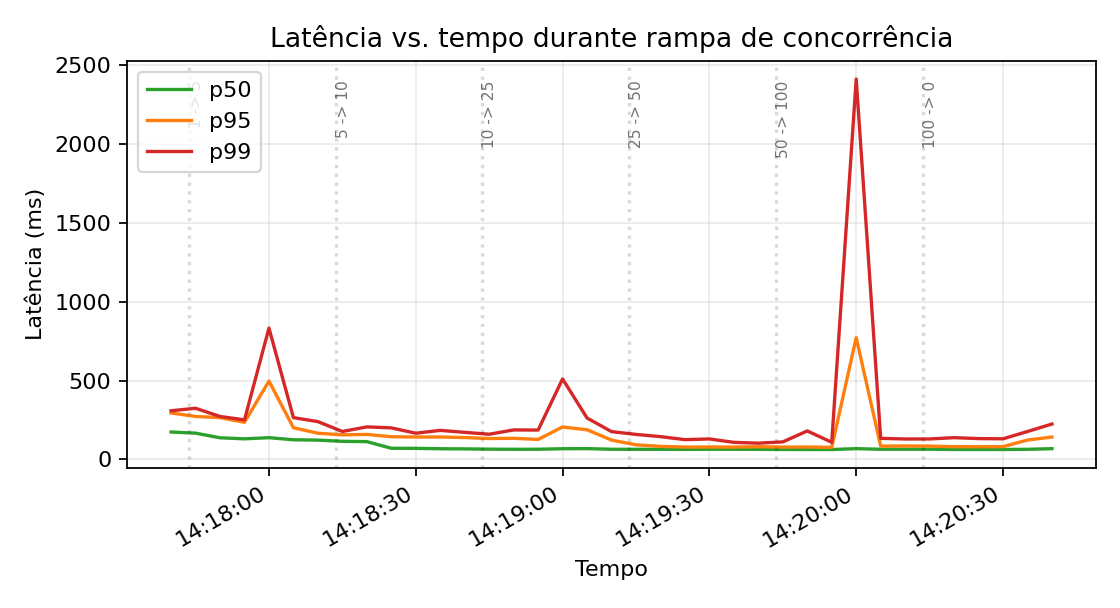
\includegraphics[width=\columnwidth]{latency_concurrent.png}
\caption{Latência ao longo do tempo durante a rampa de utilizadores virtuais. Cada linha vertical separa um \textit{stage} (30\,s) e indica o nível de VUs concorrentes nessa janela.}
\label{fig:lat-time}
\end{figure}

\textbf{Como interpretar:} cada ponto é o valor de um percentil agregado numa janela de 5 segundos. A linha verde (p50) descreve o pedido típico em cada instante; mantém-se aproximadamente constante porque metade dos pedidos não compete por recursos. A linha laranja (p95) e a vermelha (p99) representam a cauda — começam a separar-se da mediana à medida que a concorrência cresce, sinal de que uma minoria de pedidos passa a esperar atrás de outros.

A Figura~\ref{fig:lat-stages} agrega os mesmos dados por \textit{stage}, permitindo comparar de forma direta cada nível de concorrência.

\begin{figure}[t]
\centering
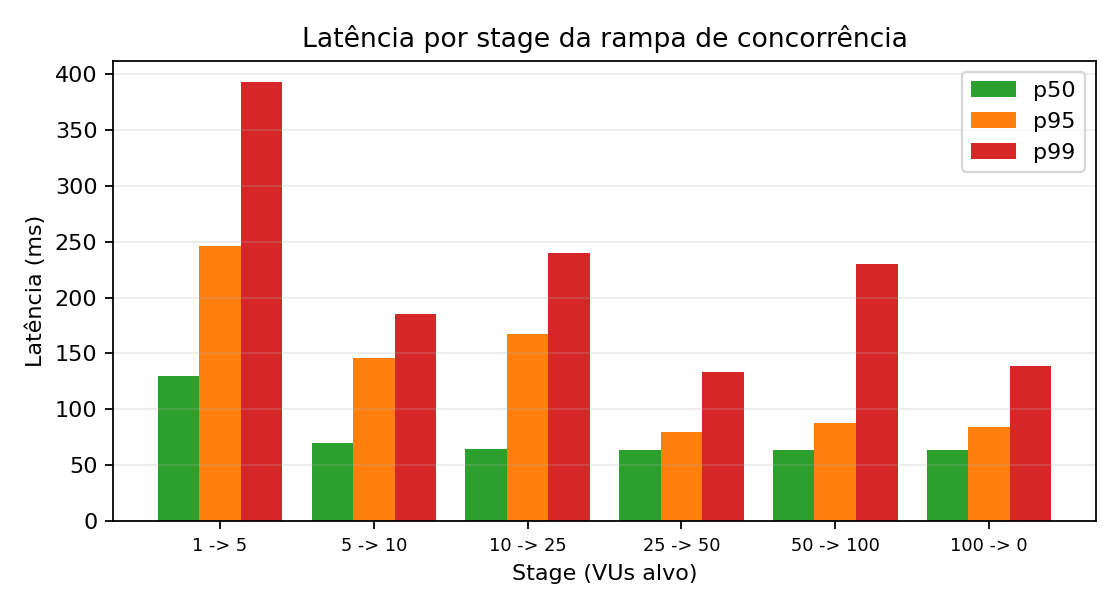
\includegraphics[width=\columnwidth]{latency_stages.png}
\caption{Latência (p50, p95, p99) agregada por \textit{stage} da rampa de concorrência. Cada grupo de três barras corresponde a uma janela de 30\,s com o nível de VUs indicado no eixo horizontal.}
\label{fig:lat-stages}
\end{figure}

\textbf{Como interpretar:} as barras verdes (p50) crescem pouco entre \textit{stages}, o que sugere que o caso típico se mantém estável mesmo com 100 utilizadores em paralelo. As barras laranja e vermelha (p95, p99) crescem de forma mais visível, sobretudo na transição para 100 VUs, indicando que a degradação se concentra na cauda da distribuição. A Tabela~\ref{tab:conc} resume os valores globais agregados sobre toda a rampa.

\begin{table}[t]
\caption{Latência concorrente, agregada sobre toda a rampa (77\,497 pedidos).}
\label{tab:conc}
\centering
\renewcommand{\arraystretch}{1.15}
\footnotesize
\begin{tabular}{@{}lrrrrrr@{}}
\toprule
\textbf{n} & \textbf{min} & \textbf{p50} & \textbf{média} & \textbf{p95} & \textbf{p99} & \textbf{max} \\
\midrule
77\,497 & 42\,ms & 64\,ms & 72\,ms & 113\,ms & 187\,ms & 9442\,ms \\
\bottomrule
\end{tabular}
\end{table}

\textbf{Observação não trivial:} os p50 e p95 do cenário concorrente são \emph{inferiores} aos do cenário sequencial. Isto é contra-intuitivo apenas à primeira leitura: como o cenário sequencial arrancou ``frio'', a sua amostra inclui o custo inicial de aquecimento dos \textit{workers}; o cenário concorrente, que corre depois, encontrou tudo pronto. O fenómeno confirma na prática a tese central do modelo: a plataforma aprovisiona capacidade sob procura e amortiza-a enquanto houver tráfego \cite{shahrad2020}. O valor máximo de 9442\,ms reflete uma pequena fração de pedidos (0{,}53\%) que apanharam \textit{rate limiting} (HTTP 429) ou reciclagem de \textit{worker} durante o pico, e não a operação normal.

\subsection{Cold Start}
O \textit{cold start} foi medido com a metodologia descrita na Secção~V-C: dez pares de pedidos (\textit{cold} + \textit{warm}), separados por intervalos de 15 minutos. A Figura~\ref{fig:cold} apresenta o resultado iteração a iteração.

\begin{figure}[t]
\centering
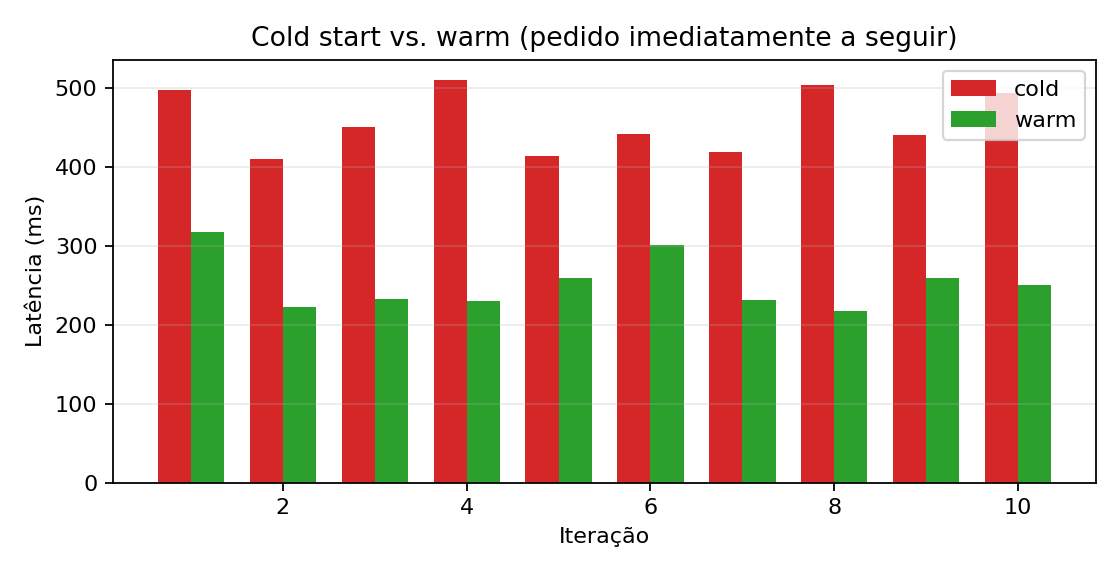
\includegraphics[width=\columnwidth]{cold_start.png}
\caption{Latência de \textit{cold start} (barra vermelha) versus \textit{warm} (barra verde) ao longo de 10 iterações espaçadas por 15 minutos. A diferença vertical entre as duas barras de uma mesma iteração corresponde ao custo de provisionamento do \textit{sandbox} Deno.}
\label{fig:cold}
\end{figure}

\textbf{Como interpretar:} cada par de barras corresponde a uma iteração do \textit{script}. A barra vermelha mede a latência total quando o \textit{worker} foi previamente reciclado (\textit{cold}); a barra verde mede o pedido seguinte, feito segundos depois sobre o \textit{worker} já provisionado (\textit{warm}). A diferença entre as duas é a melhor aproximação ao \textbf{custo de \textit{cold start}} — isto é, ao tempo extra que a primeira invocação paga por carregar o código e inicializar o \textit{runtime} Deno \cite{wang2018,manner2018}.

Verifica-se que as barras \textit{warm} são sistematicamente baixas e consistentes entre iterações, alinhando-se com a mediana do cenário sequencial aquecido. As barras \textit{cold}, em contrapartida, são várias vezes superiores. Esta penalização, observável de forma reproduzível ao longo das 10 iterações, é o trade-off direto do modelo \textit{serverless}: o utilizador beneficia da elasticidade total (incluindo escala a zero, sem custo em períodos inativos), mas paga, no primeiro pedido após inatividade, o tempo de provisionamento. Para aplicações sensíveis ao primeiro pedido, esta latência pode ser mitigada por mecanismos de \textit{warm-up} programado ou de \textit{provisioned concurrency}, ausentes do plano \textit{free} do Supabase mas comuns nas plataformas concorrentes \cite{shahrad2020}.

%=================================================================
\section{Conclusões}
%=================================================================
Este trabalho concretizou uma função \textit{serverless} para a geração de números primos inferiores a $n$, implantada nas \textit{Edge Functions} do Supabase e exposta como \textit{endpoint} HTTP global. A escolha da plataforma — justificada pela combinação de \textit{runtime} Deno, distribuição em \textit{edge} e fricção mínima de \textit{deployment} — provou ser adequada ao escopo académico e à medição experimental pretendida.

A análise quantitativa mostrou que, em regime de função aquecida, a latência mediana ronda os 65\,ms, dominada essencialmente pelo \textit{round-trip} de rede. A função escala de forma quase plana até 100 VUs concorrentes, com a maior parte da degradação a manifestar-se apenas na cauda da distribuição (p95 e p99). O \textit{cold start}, medido em condições controladas, revelou-se reproduzível e várias vezes superior à latência \textit{warm} — confirmando que continua a ser o principal compromisso do modelo FaaS.

Como trabalho futuro, valeria a pena comparar estes resultados com outra plataforma (por exemplo, Azure Functions), variar o valor de $n$ para isolar a contribuição do trabalho CPU, e explorar estratégias de mitigação de \textit{cold start} disponíveis em planos pagos do Supabase.

\begin{thebibliography}{00}

\bibitem{baldini2017} I. Baldini \textit{et al.}, ``Serverless computing: Current trends and open problems,'' in \textit{Research Advances in Cloud Computing}, S. Chaudhary, G. Somani, R. Buyya, Eds. Singapore: Springer, 2017, pp. 1--20. doi: 10.1007/978-981-10-5026-8\_1.

\bibitem{jonas2019} E. Jonas \textit{et al.}, ``Cloud programming simplified: A Berkeley view on serverless computing,'' EECS Dept., Univ. California, Berkeley, Tech. Rep. UCB/EECS-2019-3, Feb. 2019. [Online]. Disponível: \url{https://www2.eecs.berkeley.edu/Pubs/TechRpts/2019/EECS-2019-3.html}

\bibitem{castro2019} P. Castro, V. Ishakian, V. Muthusamy, e A. Slominski, ``The rise of serverless computing,'' \textit{Communications of the ACM}, vol. 62, n.º 12, pp. 44--54, dez. 2019. doi: 10.1145/3368454.

\bibitem{hellerstein2019} J. M. Hellerstein \textit{et al.}, ``Serverless computing: One step forward, two steps back,'' in \textit{Proc. 9th Biennial Conf. Innovative Data Systems Research (CIDR)}, Asilomar, CA, USA, jan. 2019.

\bibitem{wang2018} L. Wang, M. Li, Y. Zhang, T. Ristenpart, e M. Swift, ``Peeking behind the curtains of serverless platforms,'' in \textit{Proc. USENIX Annual Technical Conf. (ATC)}, Boston, MA, USA, 2018, pp. 133--146.

\bibitem{manner2018} J. Manner, M. Endreß, T. Heckel, e G. Wirtz, ``Cold start influencing factors in function as a service,'' in \textit{Proc. IEEE/ACM Int. Conf. Utility and Cloud Computing Companion (UCC Companion)}, Zurich, Switzerland, 2018, pp. 181--188. doi: 10.1109/UCC-Companion.2018.00054.

\bibitem{shahrad2020} M. Shahrad \textit{et al.}, ``Serverless in the wild: Characterizing and optimizing the serverless workload at a large cloud provider,'' in \textit{Proc. USENIX Annual Technical Conf. (ATC)}, 2020, pp. 205--218.

\bibitem{satya2017} M. Satyanarayanan, ``The emergence of edge computing,'' \textit{Computer}, vol. 50, n.º 1, pp. 30--39, jan. 2017. doi: 10.1109/MC.2017.9.

\bibitem{shi2016} W. Shi, J. Cao, Q. Zhang, Y. Li, e L. Xu, ``Edge computing: Vision and challenges,'' \textit{IEEE Internet of Things Journal}, vol. 3, n.º 5, pp. 637--646, out. 2016. doi: 10.1109/JIOT.2016.2579198.

\bibitem{supabase} Supabase, ``Edge Functions,'' 2026. [Online]. Disponível: \url{https://supabase.com/}

\bibitem{supabasequickstart} Supabase, ``Edge Functions Quickstart,'' 2026. [Online]. Disponível: \url{https://supabase.com/docs/guides/functions/quickstart}

\bibitem{deno} Deno Land Inc., ``Deno --- A modern runtime for JavaScript and TypeScript,'' 2026. [Online]. Disponível: \url{https://deno.com/}

\bibitem{k6} Grafana Labs, ``k6: Modern load testing for developers and testers,'' 2026. [Online]. Disponível: \url{https://k6.io/}

\bibitem{insomnia} Kong Inc., ``Insomnia API Client,'' 2026. [Online]. Disponível: \url{https://insomnia.rest/}

\bibitem{azurefunctions} Microsoft Azure, ``Azure Functions,'' 2026. [Online]. Disponível: \url{https://azure.microsoft.com/pt-pt/products/functions/}

\bibitem{ibmcodeengine} IBM Cloud, ``IBM Cloud Code Engine documentation,'' 2026. [Online]. Disponível: \url{https://cloud.ibm.com/docs/codeengine}

\bibitem{firebasefunctions} Google, ``Cloud Functions for Firebase,'' 2026. [Online]. Disponível: \url{https://firebase.google.com/docs/functions}

\end{thebibliography}

\end{document}
